\chapter{Chips and PEAs}

George has some comments elsewhere in this issue on the Christmas eBook in which he mentions my lack of useful uses of the \texttt{LINK}, \texttt{UNLK} and \texttt{PEA} instructions. 

I mentioned compilers earlier myself, so now is the time to combine these into an example of the use of these instructions, which were, apparently, originally designed for compiler writers to use. They are certainly useful for converting C code, for example, into assembler. Take the following \emph{slightly} contrived C code:

\begin{lstlisting}[firstnumber=1,caption={Contrived C Code}]
void addTwoNumbers(short value_a, short value_b, long *result) 
{
   long temp;
   
   temp = value_a;
   temp += value_b;
   
   *result = temp;
}

int main(int argc, char *argv[])
{
   long Answer = 0;
   short a = 27;
   short b = 33;
   addTwoNumbers(a, b, &Answer);
   printf("a=%d, b=%d, a+b=%ld", a, b, Answer);
}
\end{lstlisting}

You can see that $addTwoNumbers$ is a rather simple function that takes two values to be added together, $value\_a$ and $value\_b$, which are \texttt{short} integers, or 16 bit words in assembly speak, and a pointer to a \texttt{long} integer, $result$. $Result$ is the \emph{address} of a 32 bit long word, where the calculated value will be stored.

The two numbers to be added are passed \emph{by value}, while the result variable is passed \emph{by reference}. This means that regardless of what the function does to the variables $value\_a$ and $value\_b$, nothing will happen to them in the calling program as within the function, they are \emph{copies} of the variables rather than the actual variables themselves.

In C, if you wish to amend a variable passed as a parameter to a function, then you must pass the address of the variable - a reference to the variable in other words. Mind you, the reference is itself passed by value as a copy of the real address, so the function cannot change the address, only what it points to.

Did I mention how simple compiler writing is? (George might have some comments to make here, he is Turbo Man these days and maintains and improves the much loved Turbo Compiler and toolkit.)

Yes, I know the C code above can be rewritten to be much much simpler, and to return the actual result through the normal manner in C, using the \texttt{return} command, but bear with me, I'm trying to demonstrate the \texttt{LINK}, \texttt{UNLK} and \texttt{PEA} instructions! 

The local variable $temp$ will have space allocated on the stack for it, and when the function ends, this temporary work space will be removed. With a compiler producing code for the Motorola 68000 series of processors, the code generated \emph{could} resemble the following.

\begin{lstlisting}[firstnumber=1,caption={Contrived Assembly Code}]

main           equ *

Answer         dc.l 0
a              dc.w 27
b              dc.w 33

               lea a,a0              Get address of a.
               move.w (a0),-(a7)     Stack a's value 27.
               lea b,a0              Get address of b.
               move.w (a0),-(a7)     Stack b's value 33.
               pea Answer            Stack reference to Answer.
               bsr addTwoNumbers
Stack_tidy     adda.l #2+2+4,a7      Tidy the stack.
               ...               
\end{lstlisting}

The code for main starts with some space allocated for the variables defined within the C code. Then, a copy of the values of variables $a$ and $b$ are pushed onto the stack, followed by the address of the variable $Answer$.

After the function call, these 8 bytes are tidied off the stack, before main carries on with whatever comes next.

The \texttt{PEA} instruction is roughly equivalent to the following code:

\begin{lstlisting}[caption={PEA Equivalent Code}]
               lea Answer,a0
               move.l a0,-(a7)
\end{lstlisting}

Back to the contrived example, the assembly code created for the function, might be as follows:

\begin{lstlisting}[firstnumber=16,caption={Contrived Assembly Code - AddTwoNumbers}]
addTwoNumbers  equ *
               link a6,-4            Local variable temp.
               move.l a0,-(a7)       Save working register.
               clr.l -4(a6)          Locals default to zero.
               move.w $0e(a6),-4(a6) Get value_a.
               add.w $0c(a6),-4(a6)  Add value_b.
               move.l $08(a6),a0     Fetch address of Answer.
               move.l -4(a6),(a0)    Copy temp into Answer.
               move.l (a7)+,a0       Restore working register.
               unlk a6               Clean up temp, a6 and a7.
               rts
              
\end{lstlisting}

%  0e Value of A (27).
%  0c Value of B (33).
%  08 Address of Answer.
%  04 Return address (of Stack_tidy).
%  00 Old value of A6.l    <---- A6 = fp.
%  -4 Space for Temp.
%  -8 Daved value of A0.l  <---- A7 = sp.

This code starts by creating space, 4 bytes, for the local variable named $temp$ using the \texttt{LINK} instruction which creates a stack frame big enough to hold all the local variables required, and sets A6 to be the frame pointer. It does this \emph{effectively} as per the following code:

\begin{lstlisting}[firstnumber=1,caption={LINK Effective Code}]
               move.l a6,-(a7)       Save current a6.
               movea.l a7,a6         A6 is the frame pointer.
               adda.l #-4,a7         Create space for locals.
\end{lstlisting}

With a6 as the frame pointer, the code can access local variables using a negative offset from A6, and access the function parameters with a positive offset from A6. Any working registers pushed onto the stack will go below the space required for the local variables used in the function. At this point, the stack looks like \figurename~\ref{fig:StackFrame}


\begin{figure}[h]
\begin{center}
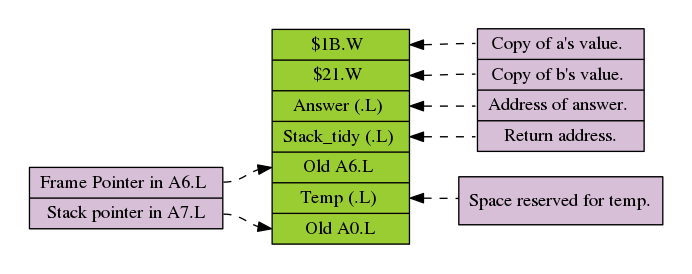
\includegraphics[scale=0.4]{images/stack.png}
\end{center}
\caption{The stack structure}
\label{fig:StackFrame}
\end{figure}
 

After setting the $temp$ local variable to zero, the calculation is done and the result stored in the long word pointed to by $result$ which is the address of the variable $Answer$, and the stack is tidied by popping A0 and then by unwinding the stack frame previously allocated using the \texttt{UNLK} instruction, which \emph{effectively}, does this:

\begin{lstlisting}[firstnumber=1,caption={UNLK Effective Code}]
               move.l a6,a7           Set a7 back again.
               move.l (a7)+,a6        Retrieve previous a6.
\end{lstlisting}

And now, A7 points once again, at the return address in main, where execution will continue. The local variable $temp$ is no more, it has ceased to be, it has shuffled off its mortal coil and gone to meet its maker, etc.\footnote{Monty Python's Dead Parrot sketch.}
